\chapter{title tbd}
kinda wanna do an intro 
\section{Categorical Background Mish Mash (title work in progress)}

\section{Background}
Okay i'm just gonna type and we'll see what comes out and I'll fix this
later. so this chapter is based off the work in john sterling's (aka johnny s) sheaf
semanticcs of noninterference. quick crash course in info flow terminology

\begin{definition}[Lattices]
A lattice $\mathcal{L}$ is a partially ordered set which has all \textit{meets} and \textit{joins}.
\begin{itemize}
    \item Two elements $l,k \in \mathcal{L}$ have a \textit{meet} if there exists an $m\in\mathcal{L}$
          such that $m$ is the greatest lower bound of $l$ and $k$. \textit{Joins} are symmetrically least upper bounds.
    \item Having all meets and joins means for any pair of elements in the lattice, you can find a greatest lower bound as well as a least upper bound.
\end{itemize}
\end{definition}
People generally refer to a lattice of security levels $\ell$ when reasoning about information flow. The simplest example is the set
$\{L,H\}$, where $L < H$, referring to low-security (public) and high-security (private) respectively.

A simple way to think about this lattice with respect to programming is by "labelling" variables with some $\ell \in \mathcal{L}$, e.g.
$x_L$ represents that $x$ is a low-security variable. Alternatively we also have security types which are implemented in a myriad of ways,
but the simplest example is that if we want talk about $x_L$ of type Int with this framework, we would say $x$ has type $Int_L$, where $Int_L$ represents
public ints.  


When working \textcolor{red}{(should confirm this is correct)} with information flow, we ideally want use of public data
to not reveal anything about secret data. The strongest statement of this is requiring that public data 
never depends on secret data, i.e., a total absence of information flow, usually referred to as noninterference. 


\begin{definition}[$\ell-$equivalence]
Two states $\sigma,\sigma'$ are $\ell$-equivalent, denoted $\sigma \sim_\ell \sigma'$, if for all $x_\ell$, we
have $\sigma(x_\ell) = \sigma'(x_\ell)$
\end{definition}

\begin{definition}[Noninterference]
    A program $\alpha$ satisfies \textit{noninterference} if, for any states $\sigma_1,\sigma_2$ such that 
    $\sigma_1 \sim_L \sigma_2$, and $\langle \sigma_1, \alpha\rangle \downarrow \sigma'_1$, 
    $\langle \sigma_2, \alpha\rangle\downarrow \sigma'_2$, we have $\sigma'_1 \sim_L \sigma'_2$.
    If initial states agree on all public values, the respective post-states should agree on all public values.
    Equivalently, the following diagram commutes:
    \[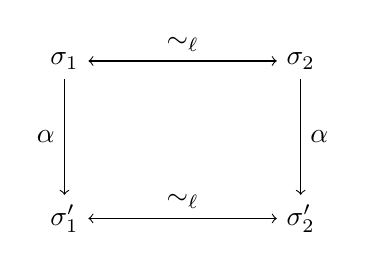
\begin{tikzpicture}
  \node (s1) at (0,2) {$\sigma_1$};
  \node (s2) at (3,2) {$\sigma_2$};
  \node (s1') at (0,0) {$\sigma'_1$};
  \node (s2') at (3,0) {$\sigma'_2$};
  
  \draw[<->] (s1) -- (s2) node[midway,above] {$\sim_\ell$};
  \draw[<->] (s1') -- (s2') node[midway,above] {$\sim_\ell$};
  
  \draw[->] (s1) -- (s1') node[midway,left] {$\alpha$};
  \draw[->] (s2) -- (s2') node[midway,right] {$\alpha$};
\end{tikzpicture}\]


    This property is also referred to as $\sigma_1$ and $\sigma_2$ being \textit{indistinguishable} with respect to public values.
\end{definition}


This indistinguishability property is equivalent to requiring any map from some type $\tau_H$ to type $\tau_L$
to be \textit{weakly constant}. A function $f: X \to Y$ is weakly constant if for any $x_1,x_2 \in X$, $f(x_1) = f(x_2)$.
One characterization of this definition is the following:
\begin{proposition}
    For any closed function $\cdot \vdash f : \tau_H \to \tau_L$, there exists a closed $\cdot \vdash v : \tau_L$ such that $f \simeq \lambda\_.v$,
    meaning $f$ is observationally (extensionally) equivalent to a constant $v$ function.
\end{proposition}

\section{categorical! almost}

Fix a poset (partially ordered set) $\mathcal{P}$ of security levels closed under finite meets. For the remainder
of this chapter we assume \[\mathcal{P} := \{L \subset M \subset H \subset \top\}.\]

%Sterling uses an Alexandroff topology, which is a structure of a topological space induced on the underlying set
%of a preordered set. 

\section{minor topological background}
\begin{definition}[Topology]
    A \textit{topology} on a set $X$ can be defined as a collection $\mathcal{T}$ of subsets of X, called \textbf{open sets} and 
    satisfying the following axioms:
    \begin{enumerate}
        \item The empty set and $X$ itself belong to $\mathcal{T}$.
        \item Any arbitrary union of members of $\mathcal{T}$ belongs to $\mathcal{T}$.
        \item The intersection of any finite number of members of $\mathcal{T}$ belong to $\mathcal{T}$.
    \end{enumerate}
\end{definition}
Technically speaking, the definition of a filter originates in topology, but a perhaps simpler and more inutitive one
exists specifically for posets, and is more relevant here.
\begin{definition}[Special Subsets]
    \begin{itemize}
        \item A \textit{filter} $\mathcal{F}$ on a poset $(\mathcal{P},\leq)$ is a subset which is upwards closed (also called an upper set). This means
    if $x \in \mathcal{F}$ and $x \leq y$, then $y \in\mathcal{F}$. Moreover, any finite subset of $\mathcal{F}$ has a lower bound.
        \item A \textit{lower set} U in $\mathcal{P}$ is downwards closed: if $x \in U$ and $z\leq x$, then $z\in U$.
    \end{itemize}
\end{definition}
Recalling that the natural numbers $\mathbb{N}$ form a poset ordered under divisibility, here is a Hasse diagram of the factors of $60$,
where the blue numbers are the elements of the upper set generated by $6$ (and in this case the upper set is also a filter), 
and the red are elements of the lower set generated by $60$.

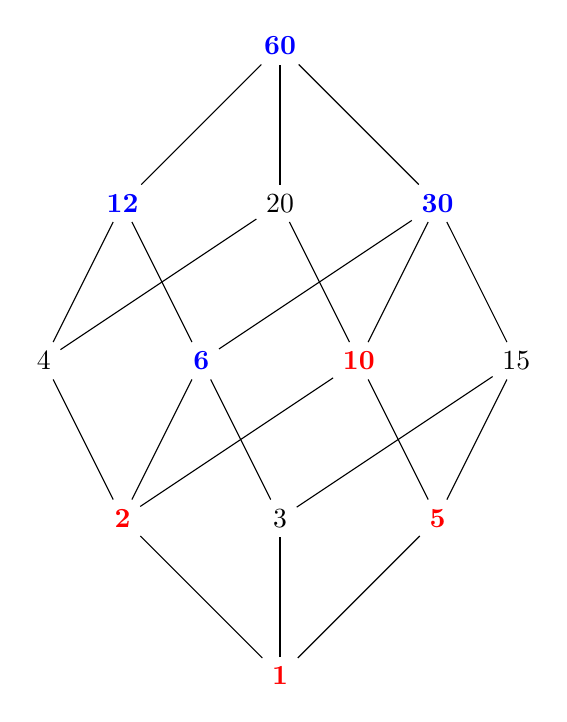
\begin{tikzpicture}
  % Level 0: 1
  \node[red] (1) at (0,0) {$\mathbf{1}$};
  
  % Level 1: prime divisors of 60
  \node[red] (2) at (-2,2) {$\mathbf{2}$};
  \node (3) at (0,2) {$3$};
  \node[red] (5) at (2,2) {$\mathbf{5}$};
  
  % Level 2: products of two primes
  \node (4) at (-3,4) {$4$};
  \node[blue] (6) at (-1,4) {$\mathbf{6}$};
  \node[red] (10) at (1,4) {$\mathbf{10}$};
  \node (15) at (3,4) {$15$};
  
  % Level 3: products of three primes
  \node[blue] (12) at (-2,6) {$\mathbf{12}$};
  \node (20) at (0,6) {$20$};
  \node[blue] (30) at (2,6) {$\mathbf{30}$};
  
  % Level 4: 60
  \node[blue] (60) at (0,8) {$\mathbf{60}$};
  
  % Edges from 1
  \draw (1) -- (2);
  \draw (1) -- (3);
  \draw (1) -- (5);
  
  % Edges from 2
  \draw (2) -- (4);
  \draw (2) -- (6);
  \draw (2) -- (10);
  
  % Edges from 3
  \draw (3) -- (6);
  \draw (3) -- (15);
  
  % Edges from 5
  \draw (5) -- (10);
  \draw (5) -- (15);
  
  % Edges from 4
  \draw (4) -- (12);
  \draw (4) -- (20);
  
  % Edges from 6
  \draw (6) -- (12);
  \draw (6) -- (30);
  
  % Edges from 10
  \draw (10) -- (20);
  \draw (10) -- (30);
  
  % Edges from 15
  \draw (15) -- (30);
  
  % Edges from 12
  \draw (12) -- (60);
  
  % Edges from 20
  \draw (20) -- (60);
  
  % Edges from 30
  \draw (30) -- (60);
  
\end{tikzpicture} 

The Alexandroff topology is a natural/induced topology on posets, where
the open sets are the upper sets. Let's check that this satisfies the axioms for open sets.
\begin{proposition}
    Upper sets of a poset $\mathcal{P}$ satisfy the following axioms:
    \begin{enumerate}
        \item The empty set and $\mathcal{P}$ itself are upper sets.
        \item Upper sets are closed under arbitrary unions.
        \item Upper sets are closed under finite intersections.
    \end{enumerate}
\end{proposition}

 \begin{proof}.
    \newline
        \begin{enumerate}
            \item $\emptyset$ as an upper set is vacuously true; there are no elements to check. For $\mathcal{P}$,
        suppose $x \in \mathcal{P}$ and $x\leq y$. Well $y\in\mathcal{P}$ because $\mathcal{P}$ is the entire set.
            \item Let $\{U_i\}_{i \in I}$ be a collection of upper sets. We wish to show $\bigcup_{i \in I} U_i$ is an upper set.
            Suppose $x \in \bigcup_{i \in I} U_i$ and $x \leq y$. Then $x \in U_j$ for some $j \in I$. $U_j$ is an upper set
            and $x\leq y$, so $y \in U_j$. Then $y \in \bigcup_{i \in I}U_i$ so arbitrary union of upper sets is also an upper set.
            \item Let $U,V$ be upper sets. We want to show $U \cap V$ is an upper set. Suppose $x\in U \cap V$ and $x\leq y$.
            Then $x \in U$ and $x \in V$. Since $U$ and $V$ are both upper sets and $x\leq y$, we have $y \in U$ and $y \in V$. Then $y \in U\cap V$!
            So upper sets are also closed under finite intersection.  
        \end{enumerate}
\end{proof}
\textit{perhaps include logical/algebraic intuition for openness axioms (knowledge / kripke semantics type)}
\newpage
\section{categorical for real}
Now we return to the original poset/lattice, $\mathcal{P} = \{L \subset M \subset H \subset T\}$.
\begin{definition}[categorical vocabulary or something]
    \begin{itemize}
        \item An \textit{abstract behavior} $x$ is a filter on the poset $\mathcal{P}$. 
        %The authors specify that $\bigwedge_{\ell_i \in \calP} \ell_i \in x$ if and only if each $\ell_i \in x$.
        We can interpret this as saying $x$
        denotes the security levels where a behavior is permitted.
        \begin{itemize}
            \item For example, a filter generated by M would include H and $\top$, capturing 
        that medium-security information/behavior can be used at higher-security levels.
        \end{itemize}
        \item A \textit{security policy} U is a lower set in $\mathcal{P}$. The notation $U \mid\vdash x$ is pronounced
        "U permits $x$", and means $U \cap x \neq \emptyset$. 
        \begin{itemize}
            \item Supposing we have a security policy generated by M, this includes L and M, and can be 
        understood as denoting the security levels \textit{above} which some information/behavior is permitted. Alternatively, 
        the set where this behavior is not allowed.
        \end{itemize}
    \end{itemize}
\end{definition}
\begin{definition}
    The authors define P to be the topological space where points are abstract behaviors, and the open sets are of the form $\{x \mid U \mid\vdash x\}$.
\end{definition}

Let's check these are open sets:
\begin{enumerate}
\item The empty set, along with being an upper set, is also a lower set (for the same vacuous reason). Then we can write the set 
$\{x \mid x \cap \emptyset \neq \emptyset\} = \emptyset$, so the empty set fits this characterization. 
Now we look at $\{ x \mid x\cap P \neq \emptyset\},$ but this in fact contains every $x$ because each $x$ is nonempty, so this set is equal to $P$.
\item Arbitrary unions: we want to write $\bigcup_{i \in I} \{x \mid U_i\mid\vdash x\}$ as \newline $\{x \mid\; ? \mid\vdash x\}$.
What does it mean for some $x'$ to be in this union? That there is some $U_j$ such that $x' \cap U_j \neq \emptyset$, which means there exists some $y$
such that $y \in x'$ and $y \in U_j$. So we can reformulate this as saying $x$ is in the arbitrary union if there exists some $j \in I$ and $y \in x$ 
such that $y \in U_j$. The existence of some $j$ can be rephrased as requiring there exist some $y\in x$ such that $y \in \bigcup_{i \in I} U_i$. Then
this is equivalent to the existence of some\newline  $y \in x \cap \bigcup_{i \in I}U_i$, so we can rewrite the arbitrary union as 
\[\{x \mid x \cap \bigcup_{i \in I}U_i\}.\]
The arbitrary union of lower sets is also a lower set --- the proof is very similar to that for upper sets, you can do it if you are not convinced. So, we have 
that these sets are closed under arbitrary unions. 
\item Finite intersections: Similarly, we can rewrite $O_V \cap O_U$ as \newline $\{x \mid (U \cap V)\mid\vdash x\}$, and lower sets are also closed under finite intersections.

\begin{proposition}
    Open sets of a space $X$ form a lattice under subset ordering, where meets are intersections $\cap$ and joins are unions $\cup$. Sometimes people refer to this behavior as the
    algebra of open sets $\mathcal{O}_X$.
\end{proposition}

Each security level $\ell \in \mathcal{P}$ represents a security policy $\langle \ell \rangle$ of the form $\{a \in \calP \mid a \leq \ell\}$. The 
corresponding open subspace of $P$, $(\{x \mid \langle \ell \rangle \mid\vdash x\})$ is denoted $P_{\langle \ell \rangle}$.

\begin{proposition}
\label{ell-in-x}
    The predicate $\langle \ell \rangle \cap x \neq \emptyset$ is equivalent to $\ell \in x$. 
\end{proposition}
To see the above, suppose we have some nonempty intersection for $\langle \ell \rangle$ and $x$. Then there exists some $k \in \langle \ell \rangle$ such that $k \in x$.
Since $k \in \langle \ell \rangle$, this means $k \leq \ell$. Since $x$ is a filter and hence upwards closed, since $\ell \geq k$ and $k \in x$, we have $\ell \in x$. 
The other direction is immediate since $\ell \in \langle \ell \rangle$ so $\ell \in x$ clearly implies a nonempty intersection. 
%This construction is an Alexandroff topology on the space of filters on $\mathcal{P}$ --- the space where the points/elements are abstract behaviors.

\begin{proposition}
    Let $\langle \ell_1 \rangle$ and $\langle \ell_2 \rangle$ be security policies such that $\ell_1 < \ell_2$. Then
    $P_{\langle \ell_1 \rangle} \subset P_{\langle \ell_2 \rangle}$.
    \begin{proof}
        Let $x$ be an abstract behavior in $P_{\langle \ell_1 \rangle}$, i.e. a filter on $\mathcal{P}$ such that ${\langle \ell_1 \rangle} \cap x \neq \emptyset$.
        Then there is some $y$ in this intersection, meaning $y \in x$ and $y \leq \ell_1$. Since $\ell_1 < \ell_2$ and posets have transitivity,
        $y < \ell_2$, which means $y \in \langle \ell_2 \rangle$. Then $y \in x \cap \langle \ell_2 \rangle$, so $x \in P_{\langle \ell_2 \rangle}$.
    \end{proof}
\end{proposition}

\section{Sheaf Interpretation}
\textit{"our intention is to interpret each type of a dependency core calculus as a sheaf on the space $P$ of abstract behaviors.
to see why this interpretation is plausible as a basis for secure information flow, we note that a sheaf on $P$ is the same thing as a presehaf on the poset 
$\mathcal{P}$"}
need to include :
\begin{itemize}
    \item mini dependency core calculus explanation (whatever is relevant)
    \item as part of above(?), using presheaves on posets for info flow
\end{itemize}

First we begin with a presheaf interpretation of information flow, where we consider the presheaf category over $\mathcal{P}$
%todo lol 

Now we parse this note : a sheaf on $P$ is "the same thing" as a presheaf on the poset $\mathcal{P}$. For someone who loves ultra precise wording, 
this remark is not very precise at all. Still, we will try to make sense of it. To me, this sounds like there is a bijection between $Sh(P)$ and $Psh(\calP)$.

\begin{theorem}
\label{P=S}
There is a bijection between the presheaf category $Psh(\calP)$ and the sheaf category $Sh(P)$.
\end{theorem}

First things first: what is sheaf, actually? 
\begin{definition}[Sheaves]
Let $\calC$ be a category with a coverage $T$. For any object $A \in \calC$, we have a T-cover $\{a_i : A_i \to A\}_{i \in I}$ indexed by some $I$. A presheaf $F$
on $\calC$ is a sheaf if it satisfies two additional conditions for \textit{any} T-cover:
\begin{enumerate}
    \item[1.] \textit{locality}: For any $f,g \in F(A)$, if $f\mid_{A_i} = g\mid_{A_i}$ for all $i \in I$, then $f = g$. If two elements agree locally 
    (on each part of the cover), they agree everywhere. We can also think of this as being able to partition any $f \in F(A)$ into the "sum of its parts", where 
    the partition / parts correspond to an arbitrary cover of $A$. 
    \item[2.] \textit{gluing}: Let $f \in F(A)$. For any $i,j \in I$, for any $x \in A_i \cap A_j$, we have $f\mid_{A_i} x = f\mid_{A_j} x$.
\end{enumerate}
\end{definition}

\begin{proposition}
\label{eq->sheaf}
    Let $\calC$ be a category with a coverage and $F : \calC^{op} \to Set$. For any $A \in \calC$, for any cover $\{a_i : A_i \to A\}$ of $A$, $F$ is a sheaf iff $F$ satisfies 
    the equalizer diagram 
  \[F(A) \xlongrightarrow{e} \prod_{i \in I} F(A_i) 
    \begin{matrix}
    \xlongrightarrow{p} \\
    \xlongrightarrow{q}
    \end{matrix}
    \prod_{i,j \in I} F(A_i \cap A_j),\]
    where $p(f_i) = f_i \mid_{A_i \cap A_j}$ and $q(f_i) = f_j \mid_{A_i \cap A_j}$.
\end{proposition}

Brief sketch on why the above is true:
\begin{lemma}
    $e$ is a monomorphism. Conversely, the morphism associated to the coequalizer is an epimorphism. These are not too hard to prove.
\end{lemma}
\begin{itemize}
    \item Since $F$ maps to \textbf{Set}, and we know \textbf{Set} is balanced, $e$ is also injective. We can think of $e$ as the map that partitions some $f \in F(A)$,
    i.e. $e(f) = \{f\mid_{A_i}\}_{i \in I}$. Then agreeing locally, $f\mid_{A_i} = g\mid_{A_i}$, is equivalent to saying $e(f) = e(g)$. Injectivity of $e$ gives us
    $f = g$.
    \item The equalizer-ness of $F$ means $F(A)$ only consists of those $f$ where $p \circ e (f) = q \circ e (f).$ We are guaranteed 
    $\left( f \mid_{A_i} \right)\mid_{A_i \cap A_j} = \left( f \mid_{A_j} \right)\mid_{A_i \cap A_j}$, which is equivalent to saying $f\mid_{A_i} x = f\mid_{A_j} x$
    for all $x \in A_i \cap A_j$.
\end{itemize}

\begin{definition}[a little more topology]
    \begin{itemize}
        \item Let $U$ be an open subset of some $S$ with topology $\calT$. The family of open sets $C = \{U_i\}_{i \in i}$ indexed by some $I$ is an \textit{open cover} of $U$
    iff $\bigcup_{i \in I}U_i = U$.
        \item A family of open subsets $\{B_i\}_{i\in I}$ of $S$ form a \textit{basis} for $\calT$ iff for any $U \subset S$, there exists some $J \subset I$ such 
        that $\{B_i\}_{i \in J}$ is an open cover of $U$. That is, any element of $\calT$ (open set) can be represented as a union of some subset of the basis elements.
    \end{itemize}
    The poset of open subsets of $S$ (ordered by inclusion) is notated $\calO(S)$. Moreover, the topological definition of a covering corresponds to a coverage on
    $\calO(S)$, where the families of morphisms are inclusion maps. 

    Taking $C$ as a cover of $U$ as above, we can write $C$ as 
    
    $\{U_i \hookrightarrow U\}_{i \in I}$.
\end{definition}

We are almost ready to begin proving \ref{P=S}.
%not sure if i want to move all of the sterling tm stuff down 

Recall the topological space at hand, $P$, has open sets of the form $\{x \mid U \mid\vdash x\}$, where $U$ is a lower set, $x$ is a filter, and 
$U \mid\vdash x$ means $U \cap x \neq \emptyset$. Note that the open sets are defined by the lower sets of $\cal P$, so we will denote them by $O_U,$ where $U$ 
is the lower set of choice. Now we have a series of lemmas.

\begin{lemma}
    The family $\{P_{\langle \ell \rangle}\}_{\ell \in \calP}$ is a basis for the topology on $P$. 
    \begin{proof}
    %i think i almost have to tbh its so far apart at this point
    We know each $P_{\langle \ell \rangle} = \{x \mid \langle \ell \rangle \mid\vdash x\}$ are open by definition. 

    Let $U$ be an upper set of $\calP$ and $O_U$ the corresponding open set of $P$, so 
    $O_U = \{x \mid x \cap U \neq \emptyset\} = \{x \mid \exists\; \ell\in\calP : \ell \in x\}$. We can tranform this into 
    \[\bigcup_{\ell \in \calP}\{x | \ell \in x\} = \bigcup_{\ell \in \calP}\{x \mid \langle \ell \rangle \mid\vdash x\} = O_U,\]
    where the second expression comes from \ref{ell-in-x}. So, we have a family of nonempty open sets of the form $P_{\langle \ell \rangle}$ indexed by some subset of 
    $\calP$ (as some of the sets in the above union will be naturally empty) such that their union is equal to $O_U$ in $P$. 
    \end{proof}
\end{lemma}
\begin{lemma}
    Let $\ell, k \in \calP$. We claim $P_{\langle \ell \rangle} \cap P_{\langle k \rangle} = P_{\langle \ell \land k\rangle}$
    \begin{proof}
        Note we have $\ell \land k$ for any $\ell,k \in \calP$ because $\calP$ is closed under finite meets. Suppose we have some $x \in P_{\langle l\land k\rangle}$,
        meaning $\ell \land k \in x$. Since $x$ is upwards closed and $\ell \land k$ is the meet of $\ell$ and $k$, it follows immediately that $\ell \in x$ and $k \in x$,
        meaning $x \in P_{\langle \ell \rangle} \cap P_{\langle k \rangle}$. 

        For the other direction, we begin with $\ell \in x$ and $k \in x$. Since $x$ is a filter, any finite subset of $x$ has a lower bound in $x$. Considering $\{\ell,k\}$
        as our subset, suppose we have some lower bound $q \in x$. By definition of meets, $q \leq \ell \land k$, so $\ell \land k \in x$,
        meaning $x \in P_{\langle \ell \land k \rangle}$. This reasoning also tells
        us that filters on a poset are closed under finite meets.
    \end{proof}
\end{lemma} 
\begin{lemma}
Any sheaf on $P$ is determined by values on the basis $\{P_{\langle \ell \rangle}\}_{\ell \in \calP}$.
\begin{proof}
    Fix some sheaf $F$ on $P$ and let $O_U$ be open in $P$. There exists some subset $\calQ \subset \calP$ 
    such that $O_U = \bigcup_{\ell \in \calQ}P_{\langle \ell \rangle}$, so $\{P_{\langle \ell \rangle}\}_{\ell \in \calQ}$ is a covering of $U$. Since $F$ is a 
    sheaf, it must satisfy
    \[F(O_U) \xlongrightarrow{e} \prod_{\ell \in \calQ} F(P_{\langle \ell \rangle}) 
    \begin{matrix}
    \xlongrightarrow{p} \\
    \xlongrightarrow{q}
    \end{matrix}
    \prod_{\ell,k \in \calQ} F(P_{\langle \ell \rangle} \cap P_{\langle k \rangle}),\]
    which is equal to 
    \[F(O_U) \xlongrightarrow{e} \prod_{\ell \in \calQ} F(P_{\langle \ell \rangle}) 
    \begin{matrix}
    \xlongrightarrow{p} \\
    \xlongrightarrow{q}
    \end{matrix}
    \prod_{\ell,k \in \calQ} F(P_{\langle \ell \land k \rangle}).\]
    %Let $s \in F(O_U)$, so $s$ can be written as a family $\{s_\ell\}_{\ell \in \calQ}$ such that $s_\ell \in F(P_{\langle \ell \rangle})$ for each $\ell \in \calQ$.
    Then to compute behavior of $F$ on $O_U$ such that the sheaf conditions are satisfied, we only need to know how $F$ acts on the basis, since we have rewritten 
    the rest of the diagram in terms of the basis elements.
\end{proof}
\end{lemma}  

Okay, now we are ready to prove \ref{P=S}!
\begin{proof}.\newline
    \begin{enumerate}
        \item $Psh(\calP) \to Sh(P)$:  
        
        Let $E$ be a presheaf on $\calP$. We will use $E$ to define a sheaf $F$ on $P$. We have the natural behavior
        for the basis elements: $F(P_{\langle \ell \rangle}) := E(\ell)$. 

        As we showed above, all the other open sets follow immediately when we set $F(O_U)$ as the equalizer of the diagram with the covering of choice being the 
        basis elements. Note that this extends to arbitrary coverings, as each open set can be written itself as a union of basis elements, so no matter what we can
        always reduce a covering to its basis elements. 
        
        F maintains all the presheaf requirements as well: suppose $P_{\langle \ell \rangle} \subset P_{\langle k \rangle}$. We've shown this implies $\ell \leq k$. 
        Then we have a restriction morphism $E(k) \to E(\ell)$, and by definition this yields a restriction morphism 
        $F(P_{\langle k \rangle}) \to F(P_{\langle \ell \rangle})$. Defining $F(O_U)$ to be the equalizer of the given diagram gives us the desired sheaf conditions, as 
        sketched in \ref{eq->sheaf}.
        \item $Sh(P) \to Psh(\calP)$:
        
        im lazy maybe i set this as a homework problem i still have to work it out. start with sheaf F. simply set $E(\ell)$ to $F(P_\ell)$ and that's all
        you need really.
    \end{enumerate}
    
\end{proof}
man oh man can you believe that was one sentence in their paper? ridiculous

if need to take up space can spice it up categorically perhaps 

\begin{definition}[Subterminal Sheaf]
    Fix a category $\calC$
    \begin{itemize}
        \item Given a functor $F$, the functor $G$ is a \textit{subfunctor} of $F$ if $G(C)\subseteq F(C) \;\forall\; C\in\calC$. If $F$ is a sheaf on $\calC$,
        then $G$ is a \textit{subsheaf} if and only if for every open $U$ of $\calC$ and every element $f \in FU$, and every open covering $U = \bigcup U_i$, one has
        $f \in SU$ if and only if $f\mid_{U_i} \in SU_i$ for all $i$.
        \item The terminal sheaf is the terminal object $\mathbf{1}$ of $Sh(\calC)$. A \textit{subterminal sheaf} $F$ is a subsheaf of 
        $\mathbf{1}$. $F$ is a subfunctor, meaning \newline $FC \subseteq \mathbf{1}C = \{*\}$ for all $C\in \calC$. This means $FC$ can only be either $\{*\}$ or $\emptyset$.      
    \end{itemize}
\end{definition}
\begin{proposition}
    A \textit{subobject} of a sheaf $F$ in the category $Sh(\calC)$ is isomorphic to a subsheaf of $F$.
    \textcolor{red}{TODO}
\end{proposition}

\begin{theorem}
    For any space $X$, there is an isomorphism \[\calO(X) \cong Sub_{Sh(X)}(\mathbf{1})\] of partially ordered sets. John Sterling will refer to this, in his
    famously precise way, as an open set of $P$ being "the same thing" as a subterminal sheaf.% in fact, of heyting algebras
    \begin{proof}(pg 73)

        Given any open set $W$ of $X$, define a functor $S_W$ on open sets $U$ by $S_W(U) = 1$ if $U\subseteq W$ and $\emptyset$ otherwise. 
        \textcolor{red}{this functor is clearly a sheaf}, so it defines a subsheaf of $\mathbf{1}$.

        Conversely, let $S$ be a subsheaf of $\mathbf{1}$. Each $S(U)$ is then either $1$ or $\emptyset$. \textcolor{red}{Since $S$ is a functor}, 
        $S(U) = 1$ for some $U$ and $V \subseteq U$ imply $S(V) = 1$. If $\{U_i\}$ is an open cover of $U$ and $SU_i = 1$ for all $i$, then 
        \textcolor{red}{by the equalizer condition}, $SU = 1$. Thus, if we let $W = \bigcup\{U \in \calO(X) \mid SU = 1\}$, then for all open sets $U$,
        $SU = 1$ iff $U \subseteq W$. That is, $S = S_W$. Thus, $W \mapsto S_W$ is the desired (order preserving) bijection.
    \end{proof}
\end{theorem}

\subsection{Transparency and Sealing Monads}
For any subspace $Q\subset P$, a sheaf $A \in Sh(P)$ can be restricted to $Q$, as in $A\mid_Q \in Sh(Q)$, and then extended again to $P$. This composite defines
an \textit{idempotent} monad on $Sh(P)$ that we can interpret as removing any data from $P$ that cannot be seen from $Q$. A monad $T$ is idempotent when $T^2 = T$
(i.e. $\mu = id$).
\begin{definition}
    \begin{enumerate}
        \item[1.] The \textit{transparency monad} $A \mapsto (\langle \ell \rangle \Rightarrow A)$ replaces $A$ with whatever part of it can be viewed under policy
        $\langle \ell \rangle$. %The transparency monad is the function space $A^{\langle \ell \rangle}$
        When the unit is an isomorphism at $A$, we say that $A$ is \textit{$\langle \ell \rangle$-transparent}.
        \item[2.] The \textit{sealing monad} $A \mapsto (\langle \ell \rangle \bullet A)$ removes from $A$ whatever part of it can be viewed under policy $\langle \ell \rangle$. 
        The sealing monad can be constructed as the pushout $\langle \ell \rangle \sqcup_{\langle \ell \rangle \times A} A.$ When the unit is an isomorphism at $A$,
        we say $A$ is \textit{$\langle \ell \rangle$-sealed}. 
    \end{enumerate}
\end{definition}

\textbf{Pushout Things/Exercises !!}
We briefly mentioned pushouts as dual to pullbacks, but it is not very intuitive to get a sense of what that means exactly.

Let's try to understand these monads through this lens of "restriction" 
%balloon diagrams to make sense of all this (or maybe not):

%Fix $A \in Sh(P)$, and recall $\calP = \{L \subset M \subset H \subset \top\}$. For our example we will work with $\langle M \rangle$. 

\end{enumerate}

